\section{Entregables}
\label{Entregables}

En esta sección se recopilan todos los resultados finales que no son simples tareas de investigación sino productos de algún tipo.

Para facilitar el acceso a estos entregables se han puesto a disposición en diferentes repositorios y en algunos casos se han desplegado interfaces con las que explorarlos o interactuar con ellos.

\subsection{Dataset en castellano}

Desde el comienzo del proyecto se determinó la necesidad de tener un dataset de voz que permitiese realizar pruebas de entrenamiento con los distintos modelos que se identificaron idóneos para cubrir las tesis de partida.

Este dataset es el resultado final tras haber experimentado con varios conjuntos algo más pequeños y haber realizado una labor de investigación sobre las características idóneas de un dataset de este tipo.

Algunas de las dificultades para la generación de este dataset se cubren en un anexo especial donde además se analizan otros datasets habituales en inglés.

El dataset generado se encuentra alojado en los siguientes repositorios de datos.

\begin{itemize}
    \item Zenodo: \url{https://zenodo.org/record/6589899}
    \item HugginFace: \url{https://huggingface.co/datasets/daniel-dona/dani-voice}
    
\end{itemize}

Estos son otros datasets más pequeños que se emplearon en algunos entrenamientos iniciales:

\begin{itemize}
    \item \url{https://huggingface.co/datasets/daniel-dona/tfg-voice-1}
    \item \url{https://huggingface.co/datasets/daniel-dona/tfg-voice-1}

\end{itemize}

\subsection{Modelo de voz propio}

El modelo generado, así como los tableros de TensorFlow con los entrenamientos se encuentran alojados en este repositorio de GitHub, así como publicados en Zenodo.

Modelo VITS final:

\begin{itemize}
    \item Sin fonemas: \url{https://doi.org/10.5281/zenodo.6589889}
    \item Usando fonemas: \url{https://doi.org/10.5281/zenodo.6589880}
\end{itemize}

Estos modelos están pensados para ser usados en el toolkit Coqui-AI, hay código de ejemplo en las interfaces de muestra que se exponen más abajo.

Otros modelos:

\begin{itemize}
    \item Modelo Tacotron2: \url{https://zenodo.org/record/6613313} y \url{https://zenodo.org/record/6613317}
\end{itemize}

\subsection{Muestras de inferencia}

Para facilitar de forma comparativa los resultados de los dos modelos, así como los dos entrenamientos distintos de VITS junto a una referencia de voz, se ha preparado una web sencilla con inferencias preparadas.

\begin{figure}[H]
\centering
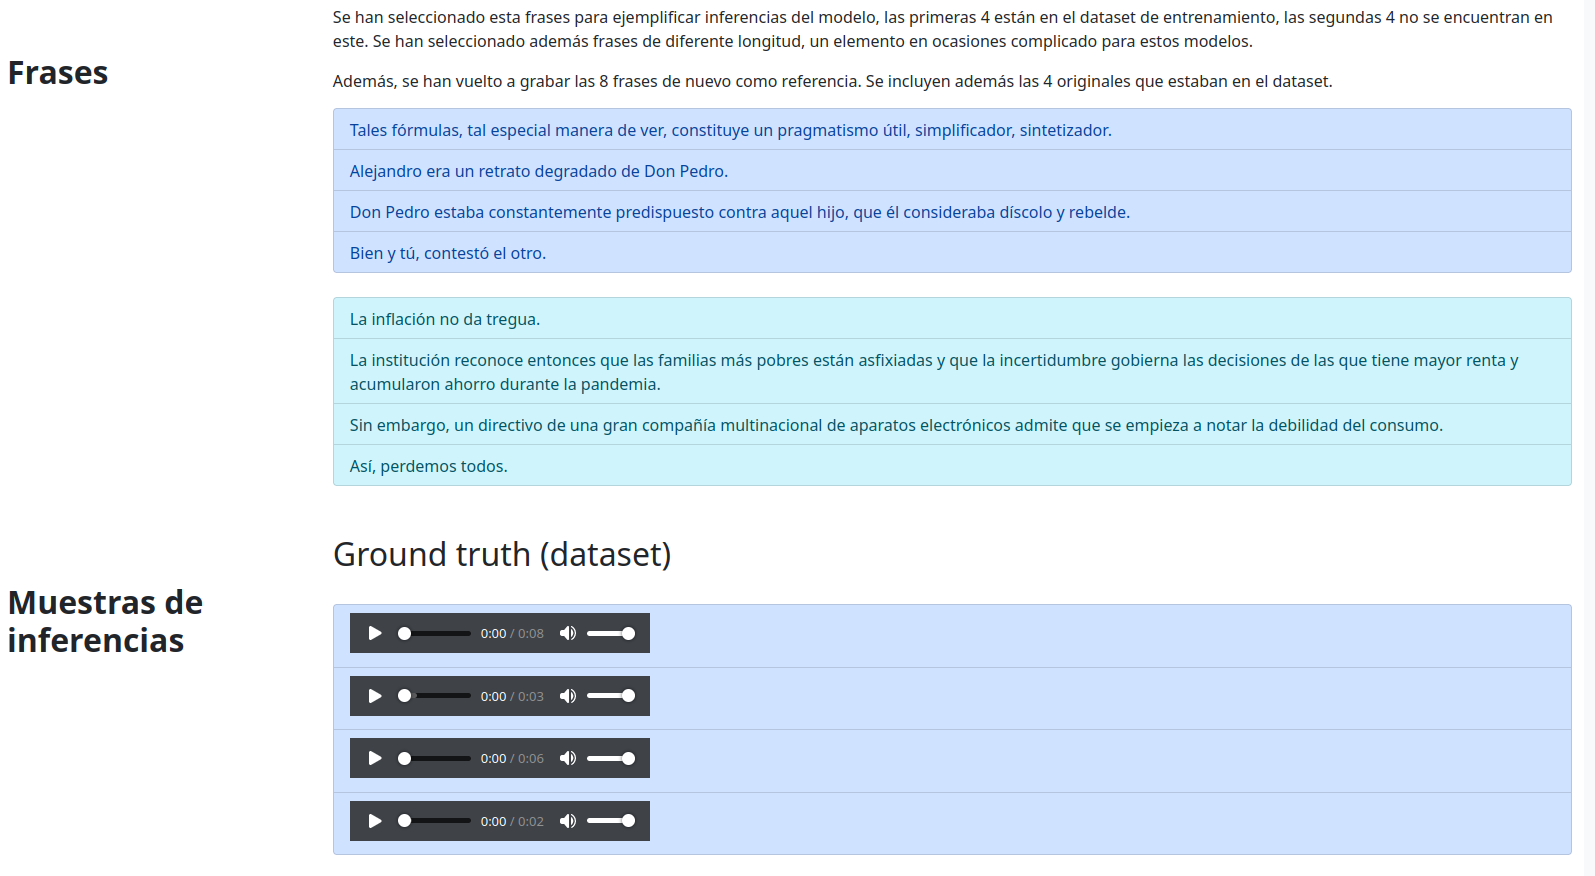
\includegraphics[width=14cm]{8_entregables_img/infer-sample-0.png}
\caption{Web con inferencias precalculadas a modo de ejemplo y comparativa.}
\label{fig:figure1}
\end{figure}


La web está disponible aquí como una simple GitHub Page: \url{https://daniel-dona.github.io/tfg-inference-samples/}


\subsection{Interfaz de pruebas}

Se han preparado varias interfaces con las que mostrar los resultados de los modelos entrenados así como permitir interactuar con ellos según se desee.

\subsubsection{Bot en Telegram}

Se trata de un usuario especial en la aplicación de chat Telegram que responde al comando /tts [texto] devolviendo una nota de voz con el resultado de la inferencia del modelo. Esta interfaz se pensó originalmente como demostración no solo de los resultados sino además de la generación en tiempo real de dichos resultados.


\begin{figure}[h]
\centering
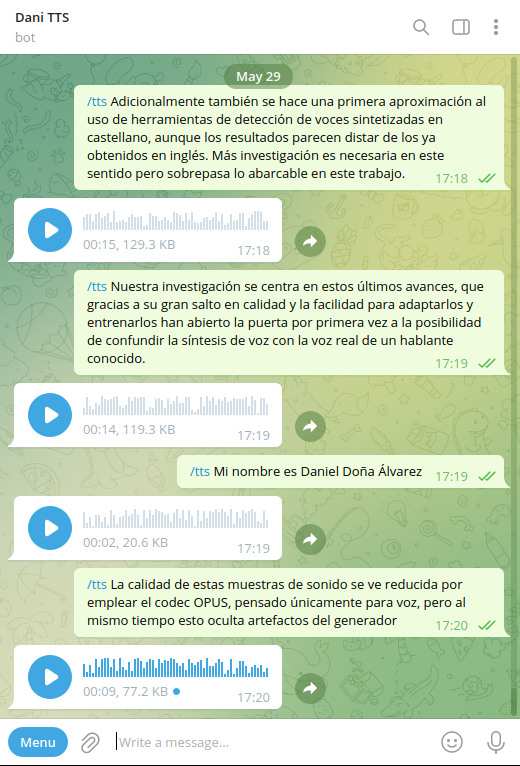
\includegraphics[width=8cm]{8_entregables_img/telegram_0.png}
\caption{Aspecto de la comunicación con el bot desplegado.}
\label{fig:figure1}
\end{figure}


Se puede interactuar con esta interfaz accediendo a esta dirección: \url{https://t.me/dani_tts_bot}

\subsubsection{Demo en HuggingFace Spaces}

HuggingFace es un ecosistema pensado para compartir datasets, modelos entrenados y demostraciones de estos modelos entre la comunidad de Aprendizaje Computacional.

Hemos desplegado una demostración del modelo también allí, estando disponible tanto su código como una interfaz sencilla para realizar inferencias.

\begin{figure}[H]
\centering
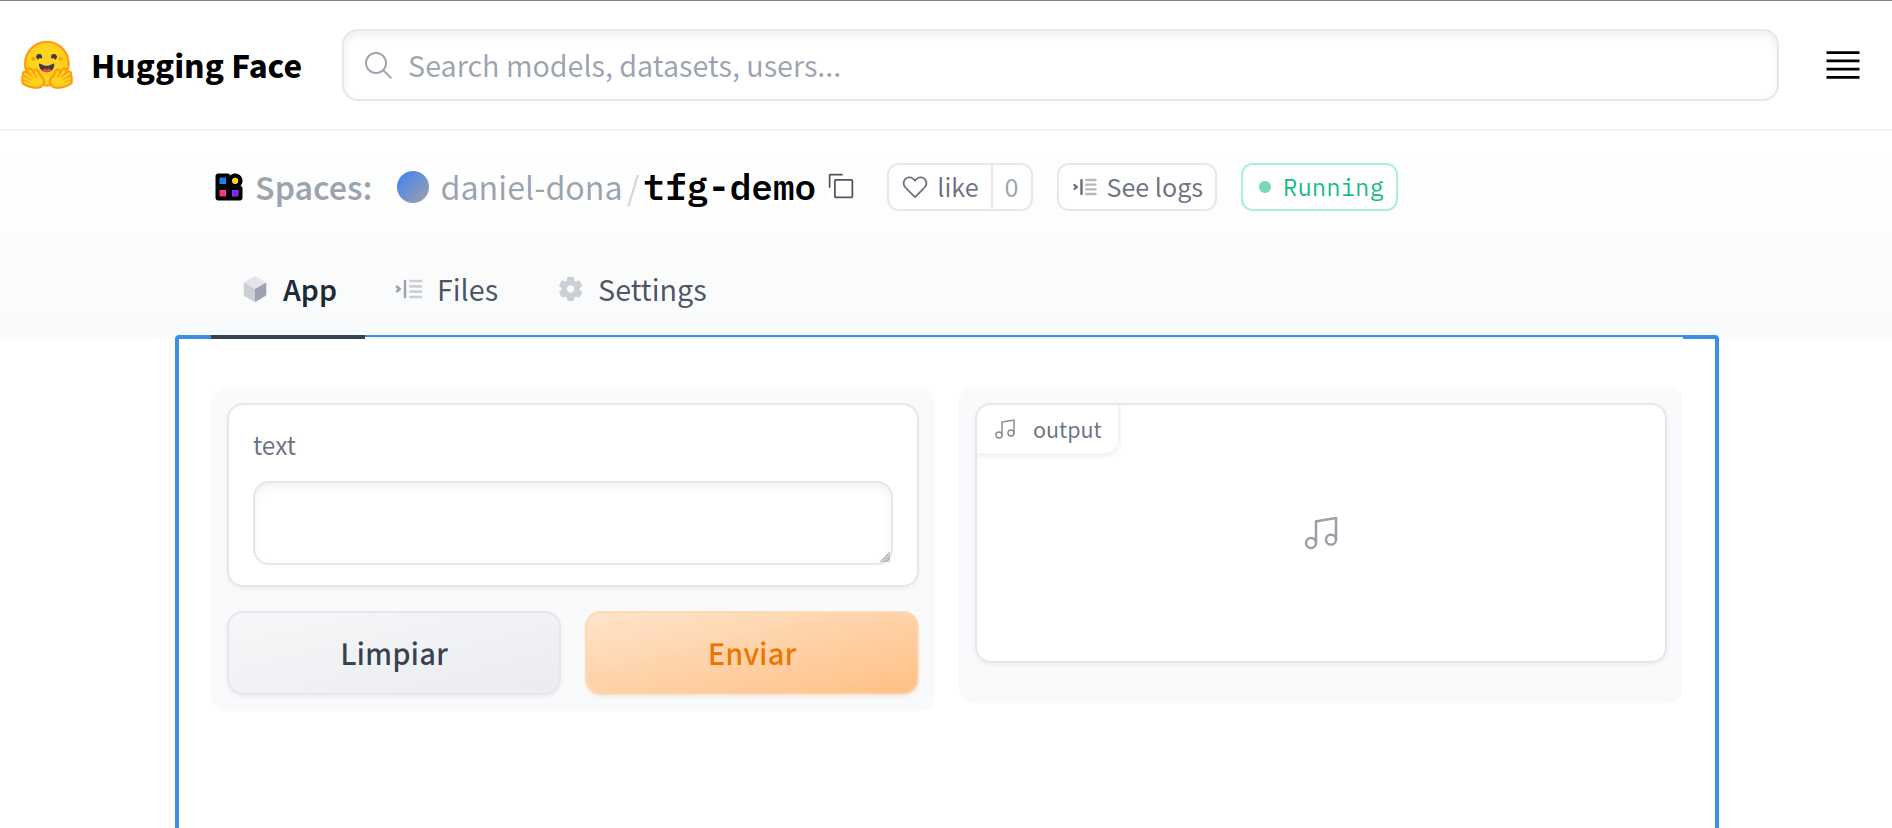
\includegraphics[width=14cm]{8_entregables_img/entrega_hf_0.png}
\caption{Interfaz de pruebas en la plataforma de HuggingFace.}
\label{fig:figure1}
\end{figure}

Se puede consultar en esta dirección: \url{https://huggingface.co/spaces/daniel-dona/tfg-demo}

\newpage 